% For printing in a4
%\documentclass[a4,10pt,twoside,openright,italian,english]{book}% twoside!

% For printing with the A5 format
\documentclass[10pt,twoside,openright,english,italian]{book}% twoside!

% Set paper size
\usepackage[twoside=true]{geometry}

%For printing with the weird format
\geometry{
	paperwidth=17cm,
	paperheight=24cm,
	margin=2cm,
	top=2.3cm,
	bindingoffset=0.4cm
}
% For printing in a4
%\geometry{a4paper,
%  margin=3cm,
%  top=3.8cm,
%  bindingoffset=0.4cm
%}

%Uncomment this for final prints: this just enables printing on a4 paper
\usepackage[cam,center,a4,pdflatex,axes]{crop}

\usepackage{phdthesis}

\usepackage{fancyhdr}
\usepackage{color}
\usepackage{array}
\usepackage{mdwmath}
\usepackage{mdwtab}
\usepackage{amsmath,amssymb}
\usepackage{cite}
\usepackage{graphicx}
\usepackage{glossaries}
\usepackage{listings}
\usepackage{subfig}
\usepackage{booktabs}
\usepackage{latexsym}
\usepackage{color}
\usepackage{url}
\usepackage{bnf}
\usepackage{rotating}
\usepackage{multirow}
\usepackage{phdtitle}
\usepackage{paralist}
\usepackage{bibentry}
%\usepackage[algochapter]{algorithm2e}
\usepackage[bookmarks=true,pdftex=false,bookmarksopen=true,pdfborder={0,0,0}]{hyperref}
\usepackage{lscape}
\usepackage{algorithmic}
\usepackage{algorithm}
\usepackage{longtable}
\usepackage[T1]{fontenc} 
\usepackage[latin1]{inputenc}

%% \hyphenation{} is used to force the 
\hyphenation{}

\newtheorem{Definition}{Definition}[section]

\lstset{tabsize=2,basicstyle=\footnotesize,breaklines=true}

\usepackage[greek,english,italian]{babel}

\usepackage{ulem}
\normalem

\hypersetup{pdftitle={Title}, pdfauthor={Author}}

\nobibliography*

\department {Department XXX}
\phdprogram{Doctoral Programme In YXYX}

\author{Name Surname}
\title{Title}
\supervisor{Supervisor Name}
\tutor{Tutor Name}
\supervisor{Coordinator Name}
\titleimage{img/logopoli.png}
\phdcycle{Year -- Cycle}

%%%%%%%%%%%%%%%%%%%%%%%%%%%%%%%%%%%%%%
% Let's Start The Real Document
%%%%%%%%%%%%%%%%%%%%%%%%%%%%%%%%%%%%%%
\begin{document}
\selectlanguage{english}

\maketitle

\pagestyle{empty}

\cleardoublepage
\newpage

%%%%%%%%%%%%%%%%%%%%%%%%%%%%%%%%%%%%%%
% Acknowledgement
%%%%%%%%%%%%%%%%%%%%%%%%%%%%%%%%%%%%%%
%Acknowledgements.


\cleardoublepage
\newpage

\pagestyle{fancy}
% change numbering into Roman numbers for the introductory part
\setcounter{page}{1}
\pagenumbering{Roman}

%%%%%%%%%%%%%%%%%%%%%%%%%%%%%%%%%%%%%%
% Abstract
%%%%%%%%%%%%%%%%%%%%%%%%%%%%%%%%%%%%%%
\chapter*{Abstract}
\lettrine{T}{he} recent exponential growth of Reinforcement Learning (RL) research has been made possible by the comparable significant improvement in computational power. Indeed, the advent of powerful and relatively affordable hardware, in particular Graphics Processing Units (GPUs), allowed researchers to extend the study of RL methodologies to highly-dimensional problems that were unpractical before, opening the line of research that is now commonly known under the name of Deep Reinforcement Learning (DRL). However, the groundbreaking results that DRL is achieving are obtained at the cost of a huge amount of samples needed for learning, along with very large learning times usually in the order of days. One of the reasons why this is happening, besides the outstanding significance of the obtained results that fundamentally poses the problems of the efficiency of these methodologies in the background, relies on the fact that often experiments are run in simulations in which the sample efficiency problem is not such an issue as in real applications. Nevertheless, an effort to improve the sample efficiency and other issues of many DRL algorithms, e.g. stability of learning, has been done by several recent works that proved to be able to address this problem successfully.

The purpose of this thesis is to study the previously described problems, which are classic issues of RL and not only of DRL, proposing novel methodologies that explicitly consider the concept of \textit{uncertainty} to speed up learning and improve its stability. Indeed, since a relevant goal of an RL agent is to reduce uncertainty about the environment in which it is moving, taking uncertainty explicitly into account can be intuitively an effective way of acting. This solution is not new in RL research, but there is still a lot of work that can be done in this direction and this thesis takes inspiration from the available literature on the subject extending it with novel significant improvements on the state of the art. In particular, the works included in this thesis can be grouped into two parts: one where uncertainty is used to improve the behavior of the Bellman equation and the other where it is used to improve exploration. The works belonging to the former group aim to address some of the problems of action-value estimation in the context of value-based RL, in particular in the estimate of the maximum operator involved in the famous $Q$-Learning algorithm and more generally in the estimate of the components of the Bellman equation. On the other hand, the works belonging to the latter group study different methodologies to improve exploration by studying the use of Thompson Sampling in RL or by introducing a variant of the Bellman equation that incorporates an optimistic estimate of the action-value function to improve exploration according to the principle of Optimism in the Face of Uncertainty (OFU).

All the works presented in this thesis are described, theoretically studied, and eventually, empirically evaluated on several RL problems. The obtained results highlight the benefits that the explicit exploitation of uncertainty in RL algorithms can provide; indeed, we show how in a large set of problems that have been chosen in order to highlight particular aspects we were interested in, e.g. exploration capabilities, our methods prove to be more stable and faster to learn than others available in the literature.


%%%%%%%%%%%%%%%%%%%%%%%%%%%%%%%%%%%%%%
% Riassunto
%%%%%%%%%%%%%%%%%%%%%%%%%%%%%%%%%%%%%%
\selectlanguage{english}
\chapter*{Summary}
\lettrine{S}{ummary} goes here.

\selectlanguage{english}

%%%%%%%%%%%%%%%%%%%%%%%%%%%%%%%%%%%%%%
% TOC
%%%%%%%%%%%%%%%%%%%%%%%%%%%%%%%%%%%%%%
\tableofcontents
\cleardoublepage
\newpage

% Now lets go back to normal numbering
\setcounter{page}{1}
\pagenumbering{arabic}

\cleardoublepage
\chapter{Title chapter 1}

%============================= INTRODUCTION =================================
\section{Introduction}\label{sec:i}
Remember that wherever you want you can cite with \verb.\cite{a1}. \cite{a1}, \cite{b1} and/or \cite{m1} someone.
Or use \verb.\footnote{That's a footnote}. like this\footnote{That's a footnote} 
% this is used to include other .tex files in order to split a long document 

%============================= SECTIONS =================================

\section{New section}
You can insert a definition
	\begin{Definition}
		PoliMi: Politecnico di Milano
	\end{Definition}
	
\section{Another section}
	\subsection{And a subsection}
		In this sub section I will include many images just to make the list of figures meaningful.

			\begin{figure}[h!tb]
				\centerline {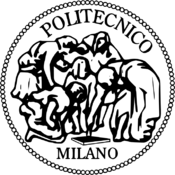
\includegraphics[scale=0.6]{img/logopoli.png}}
				\caption{Caption of this PoliMi image.}
				\label{fig:leet}
			\end{figure}

\section{New section}
	\subsection{And also many sub}
		\subsubsection{Or again more nested}
			\begin{itemize}
				\item item 1
				\item item 2
				\item item 3
			\end{itemize}			
			
\section{New section}
This is an example of table. You can see it in Table~\ref{tab:TableName}. 

 \begin{table}[h!tb]
   \centering \caption{Table caption}
   \label{tab:TableName}
   \vskip 0.2cm
   %%
   \scalebox{0.90}{
	    %% The {|c|c|c|c|c|} define the number of columns.
	    %% c means centered
	    %% | defines a vertical line between two columns 
	    \begin{tabular}{|c|c|c|}
	      \hline
	      Col 1 & Col 2 & Col2  \\
	      %% \\ force a newline without creating an horizontal line
	      Dim C.1 & Dim C.3 & Dim C.3 \\
	      %% \hline create an horizontal line between two rows
	      \hline
	      Data 1.1 & Data 1.2 & Data 1.3 \\
	      \hline
	      Data 2.1 & Data 2.2 & Data 2.3 \\
	      \hline
	      Data 3.1 & Data 3.2 & Data 3.3 \\  
	      \hline
	    \end{tabular}
	 }
 \end{table}

\section{You can do as many section as you want}
The following equation has been created using \verb.$$.: $ y_1 = a*x + b$.

%% \smallskip introduces a small vertical skip
\smallskip

%% \noindent is used to eliminate the blankline and the paragraph settings 
\noindent
This is a more complex equation: \[ y_2 = a*x + b \], created using \verb.\[ \].

%% \bigskip introduces a big vertical skip
\bigskip

\noindent
This is, (\ref{eq:eeq1}), an enumerated equation: 

	\begin{equation}\label{eq:eeq1}
		y_3 = a*x + b
	\end{equation}

, created using:

	\begin{verbatim}
		\begin{equation}\label{eq:eeq1}
		    y_3 = a*x + b
		\end{equation}
	\end{verbatim}

 % uncomment if you want part I

%\cleardoublepage
%\listoffigures
%\listoftables

\cleardoublepage
\phantomsection
\addcontentsline{toc}{chapter}{\bibname}
\small
\bibliographystyle{plain}
\bibliography{thesis}

\end{document}
